%! Author = ibw
%! Date = 09.11.23

% Preamble
%\begin{landscape}
%\storeareas\noraml
%\begin{samepage}
\clearpage
\KOMAoptions{paper=A3,paper=landscape,pagesize,DIV=20}
\recalctypearea
%\begin{landscape}
\begin{samepage}
\chapter{Projektmanagement}
\section{Projektplanung}
%! Author = gramic
%! Date = 29.02.24

% Preamble
%\begin{landscape}
\begin{flushleft}
\clearpage
\KOMAoptions{paper=A3,paper=landscape,pagesize,DIV=20}
\recalctypearea
\pagestyle{headings}
%    \clearpage
%    \KOMAoptions{paper=A3,paper=landscape,pagesize,DIV=20}
%    \recalctypearea
    \chapter{Projektmanagement}
    \section{Projektplanung}
    \subsection{Projektcontrolling}
    \begin{table}[H]

\resizebox{\columnwidth}{!}{%

\begin{tabular}{lllrrr}
\toprule
 & Phase & Subphase & Dauer [h] & Geplante Dauer [h] & Verbleibende Zeit [h] \\
\midrule
0 & 1. Expertengespräch & 1. Expertengespräch & 1.0 & 1.0 & 0.0 \\
1 & 2. Expertengespräch & 2. Expertengespräch & 1.2 & 1.0 & -0.2 \\
2 & Aufbau und Implementation Testsystem & Basisinfrastruktur & 3.0 & 4.0 & 1.0 \\
3 & Aufbau und Implementation Testsystem & Installation und Konfiguration PostgreSQL HA Cluster & 20.0 & 20.0 & 0.0 \\
4 & Aufbau und Implementation Testsystem & Technical Review & 2.0 & 3.0 & 1.0 \\
5 & Dokumentation & Dokumentation & 44.8 & 80.0 & 35.2 \\
6 & Evaluation & Analyse PostgreSQL HA Cluster Lösungen & 51.2 & 16.0 & -35.2 \\
7 & Evaluation & Anorderungskatalog & 4.5 & 16.0 & 11.5 \\
8 & Evaluation & Gegenüberstellung & 0.5 & 8.0 & 7.5 \\
9 & Evaluation & Variantenentscheid & 1.0 & 4.0 & 3.0 \\
10 & Evaluation & Vorbereitung Benchmarking & 5.0 & 4.0 & -1.0 \\
11 & Letztes Expertengespräch & Letztes Expertengespräch & 0.0 & 1.0 & 1.0 \\
12 & Puffer & Puffer & 0.0 & 16.0 & 16.0 \\
13 & Resultate & Persönliches Fazit & 0.0 & 2.0 & 2.0 \\
14 & Resultate & Schlussfolgerung & 0.0 & 2.0 & 2.0 \\
15 & Resultate & Weiteres Vorgehen / offene Arbeiten & 0.0 & 1.0 & 1.0 \\
16 & Resultate & Zielüberprüfung & 1.0 & 2.0 & 1.0 \\
17 & Testing & Protokollierung & 0.0 & 4.0 & 4.0 \\
18 & Testing & Review und Auswertung & 2.2 & 2.0 & -0.2 \\
19 & Testing & Testing Testsystem & 6.2 & 8.0 & 1.8 \\
20 & Troubleshooting und Lösungsfindung & Troubleshooting und Lösungsfindung & 11.0 & 8.0 & -3.0 \\
Total &  &  & 154.8 & 203.0 & 48.2 \\
\bottomrule
\end{tabular}
}
\caption{Projektcontrolling} \label{projektcontrolling}
\end{table}

\end{flushleft}
\clearpage
\KOMAoptions{paper=A4,paper=portrait,pagesize}
\recalctypearea
\begin{flushleft}
%\clearpage
%\KOMAoptions{paper=A4,paper=portrait,pagesize}
%\recalctypearea
\pagestyle{headings}
%\begin{flushleft}
%    \begin{figure}[H]
%        \centering
%        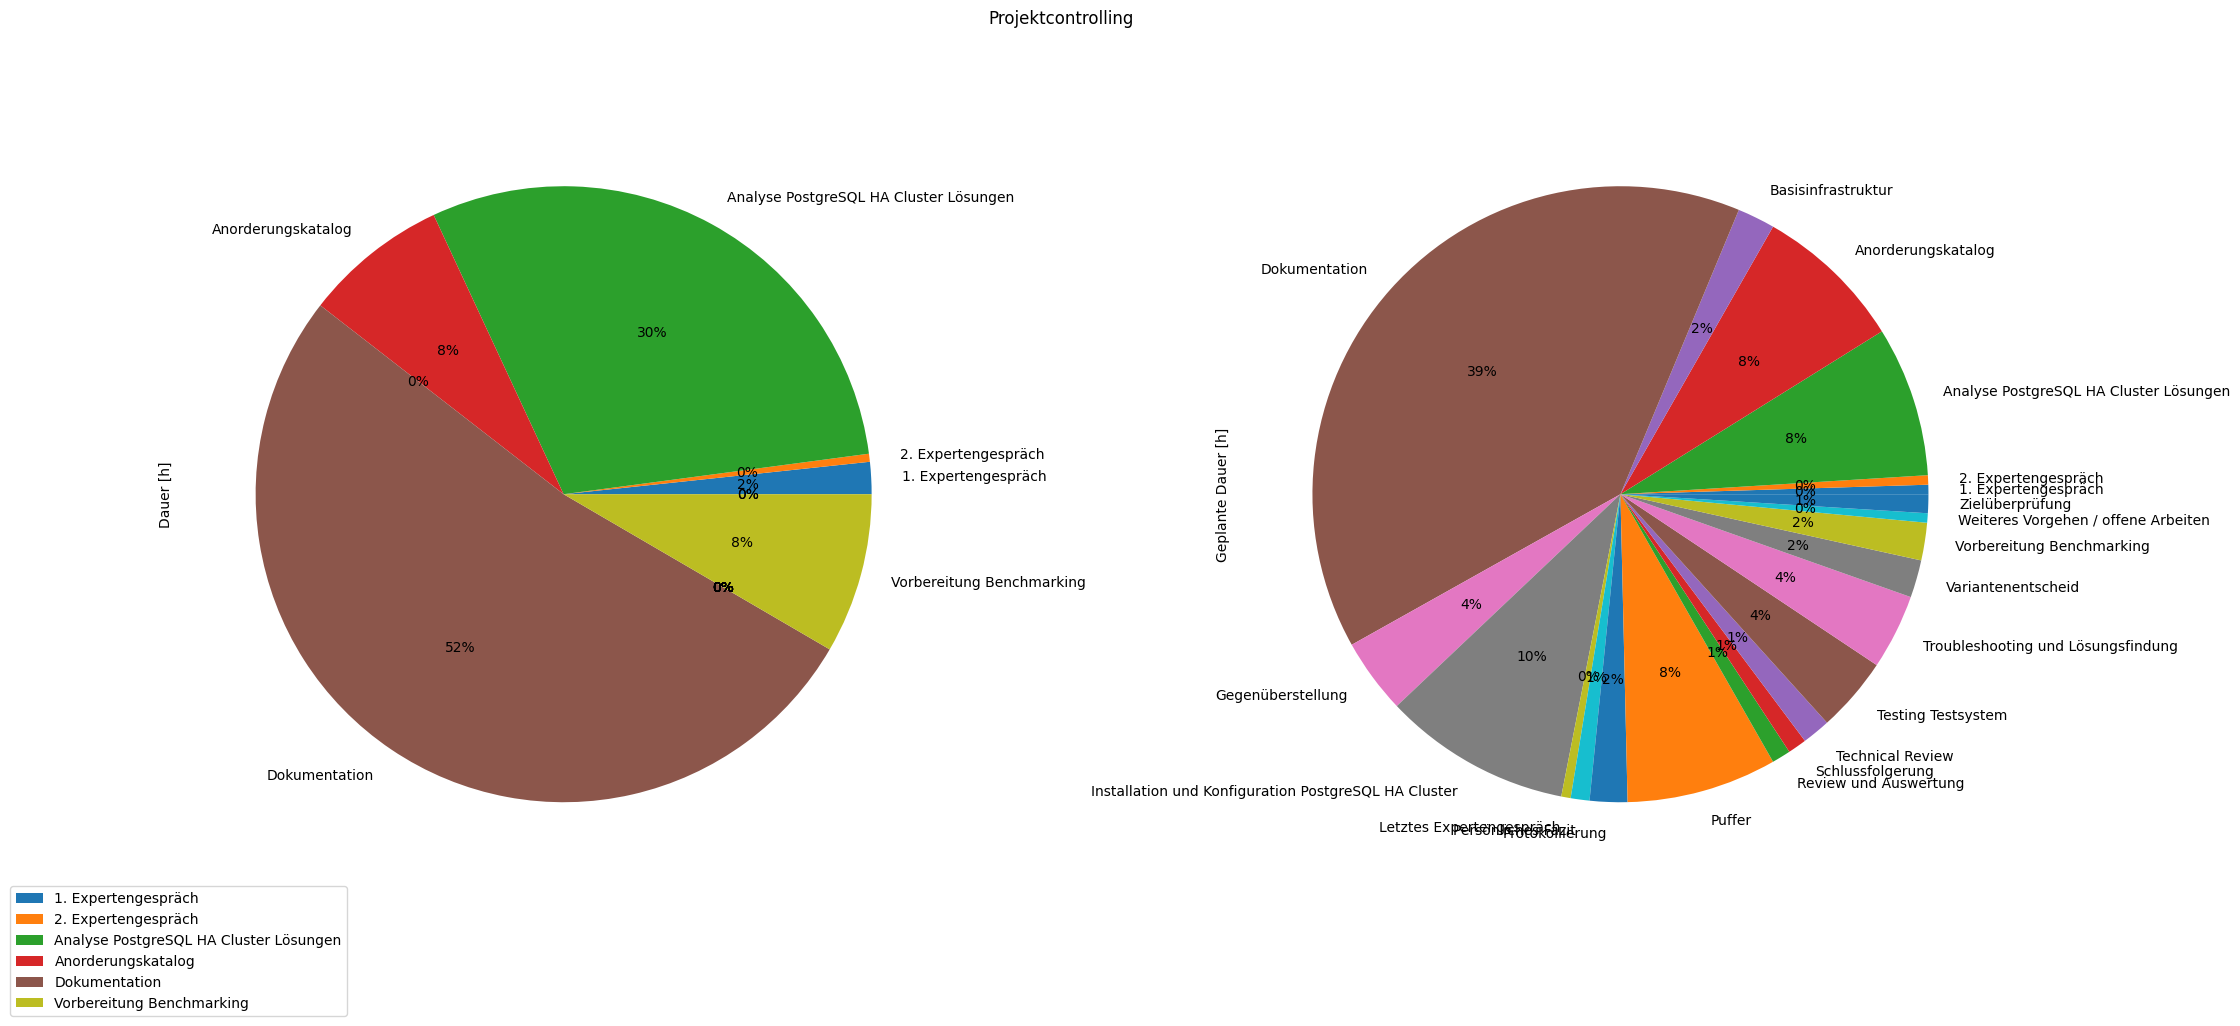
\includegraphics[width=0.75\linewidth]{source/pandas_data_chart_plotter/projektcontrolling}
%        \caption{Projektcontrolling}
%        \label{fig:projektcontrolling}
%    \end{figure}
    \begin{figure}[H]
        \centering
        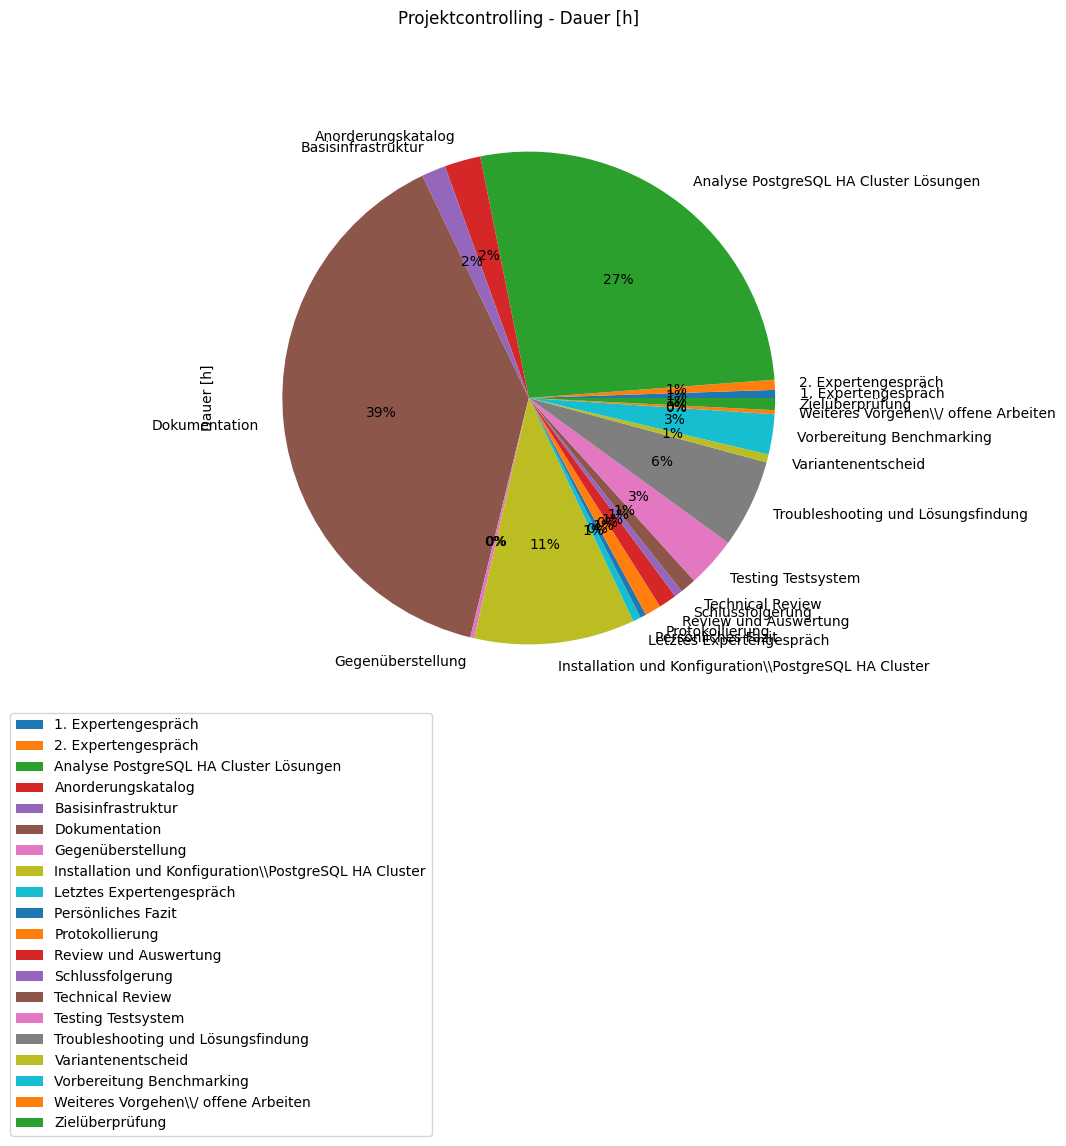
\includegraphics[width=0.75\linewidth]{source/pandas_data_chart_plotter/projektcontrolling_dauer}
        \caption{Projektcontrolling - Dauer}
        \label{fig:projektcontrolling_dauer}
    \end{figure}
\end{flushleft}
\begin{flushleft}
\clearpage
\KOMAoptions{paper=A4,paper=portrait,pagesize}
\recalctypearea
    \begin{figure}[H]
        \centering
        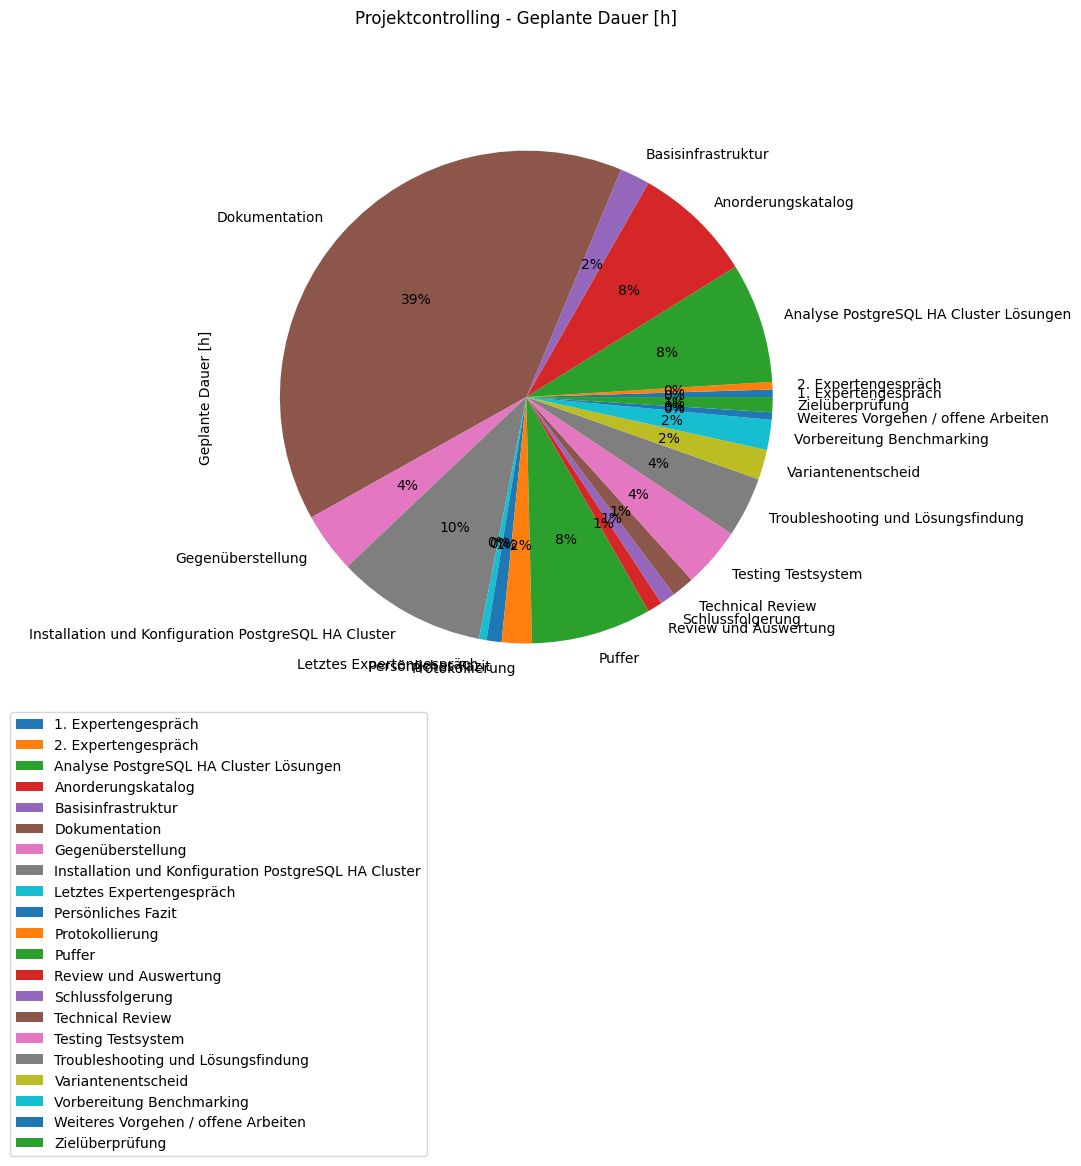
\includegraphics[width=0.75\linewidth]{source/pandas_data_chart_plotter/projektcontrolling_geplant}
        \caption{Projektcontrolling - Geplante Dauer}
        \label{fig:projektcontrolling_geplant}
    \end{figure}
\end{flushleft}
\clearpage
%\end{landscape}
\end{samepage}

%\starttext
%\setuppapersize[A3,landscape]
%\KOMAoptions{paper=A3,paper=landscape,DIV=20}
%\subsection{GANTT-Diagramm}
%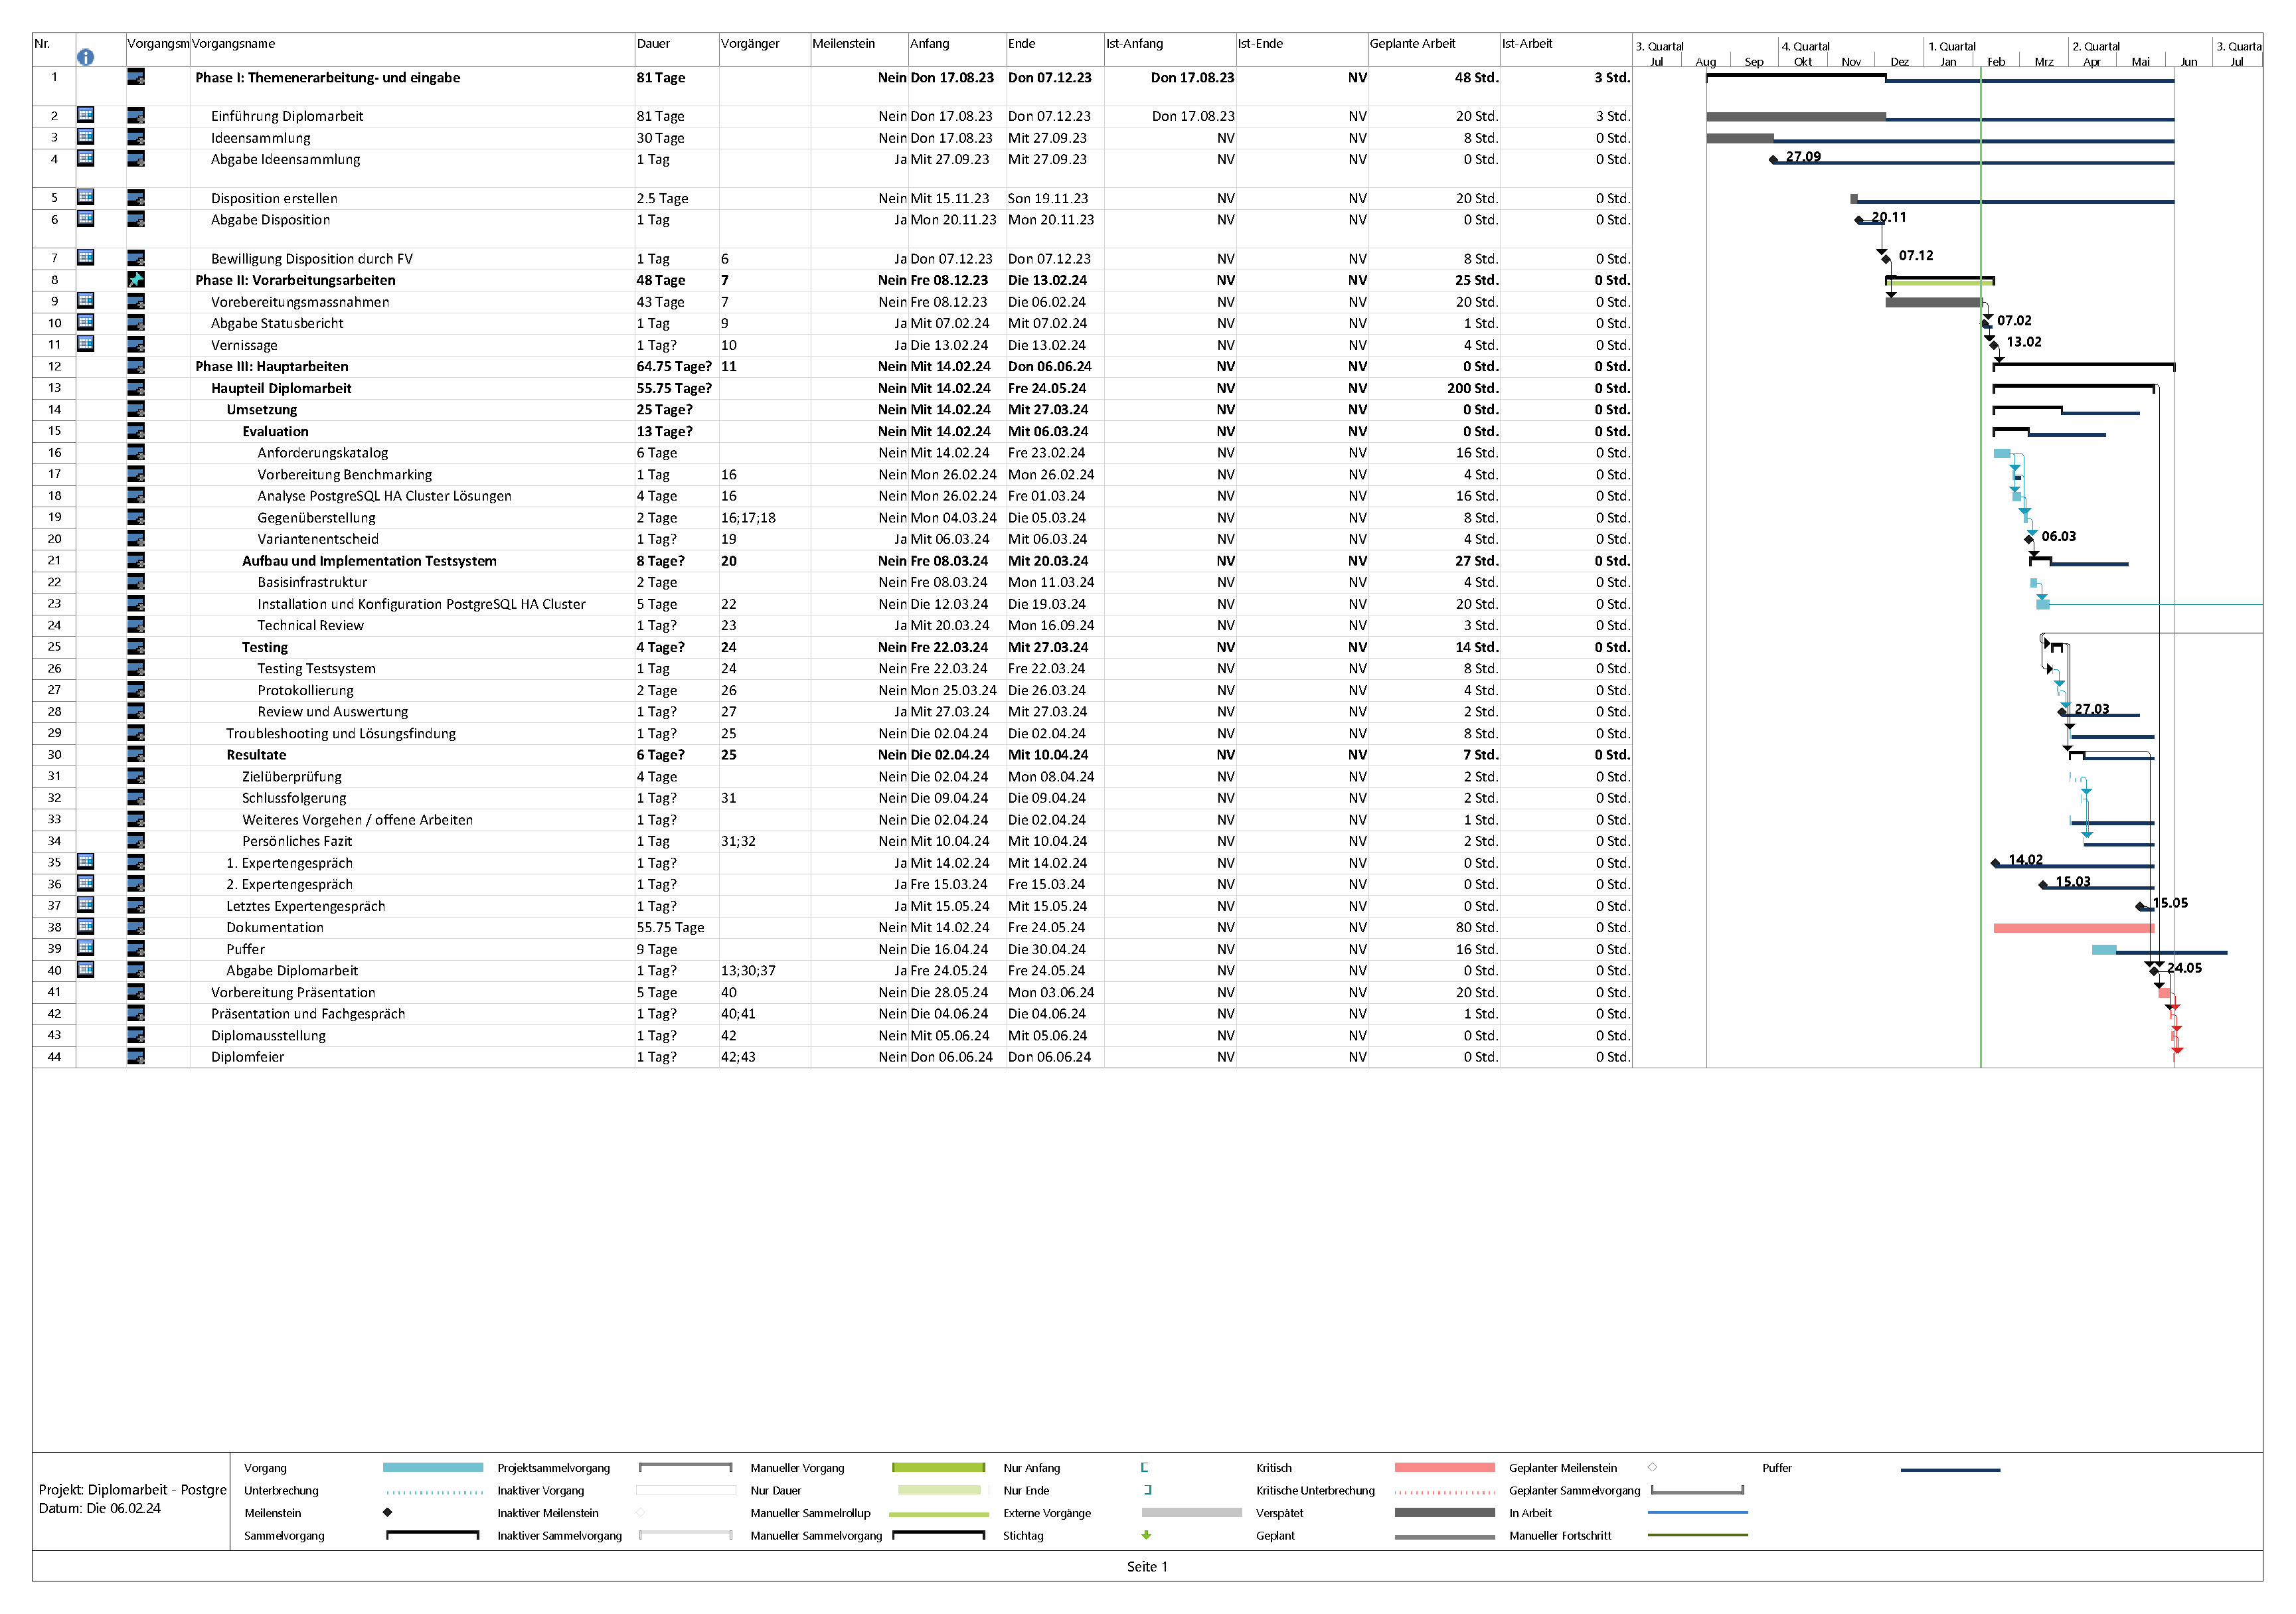
\includepdf[pages={1-},scale=1,landscape=true]{source/status_report/main/Diplomarbeit_PostgreSQL_HA_Cluster_Konzeption_und_Implementation.pdf}
%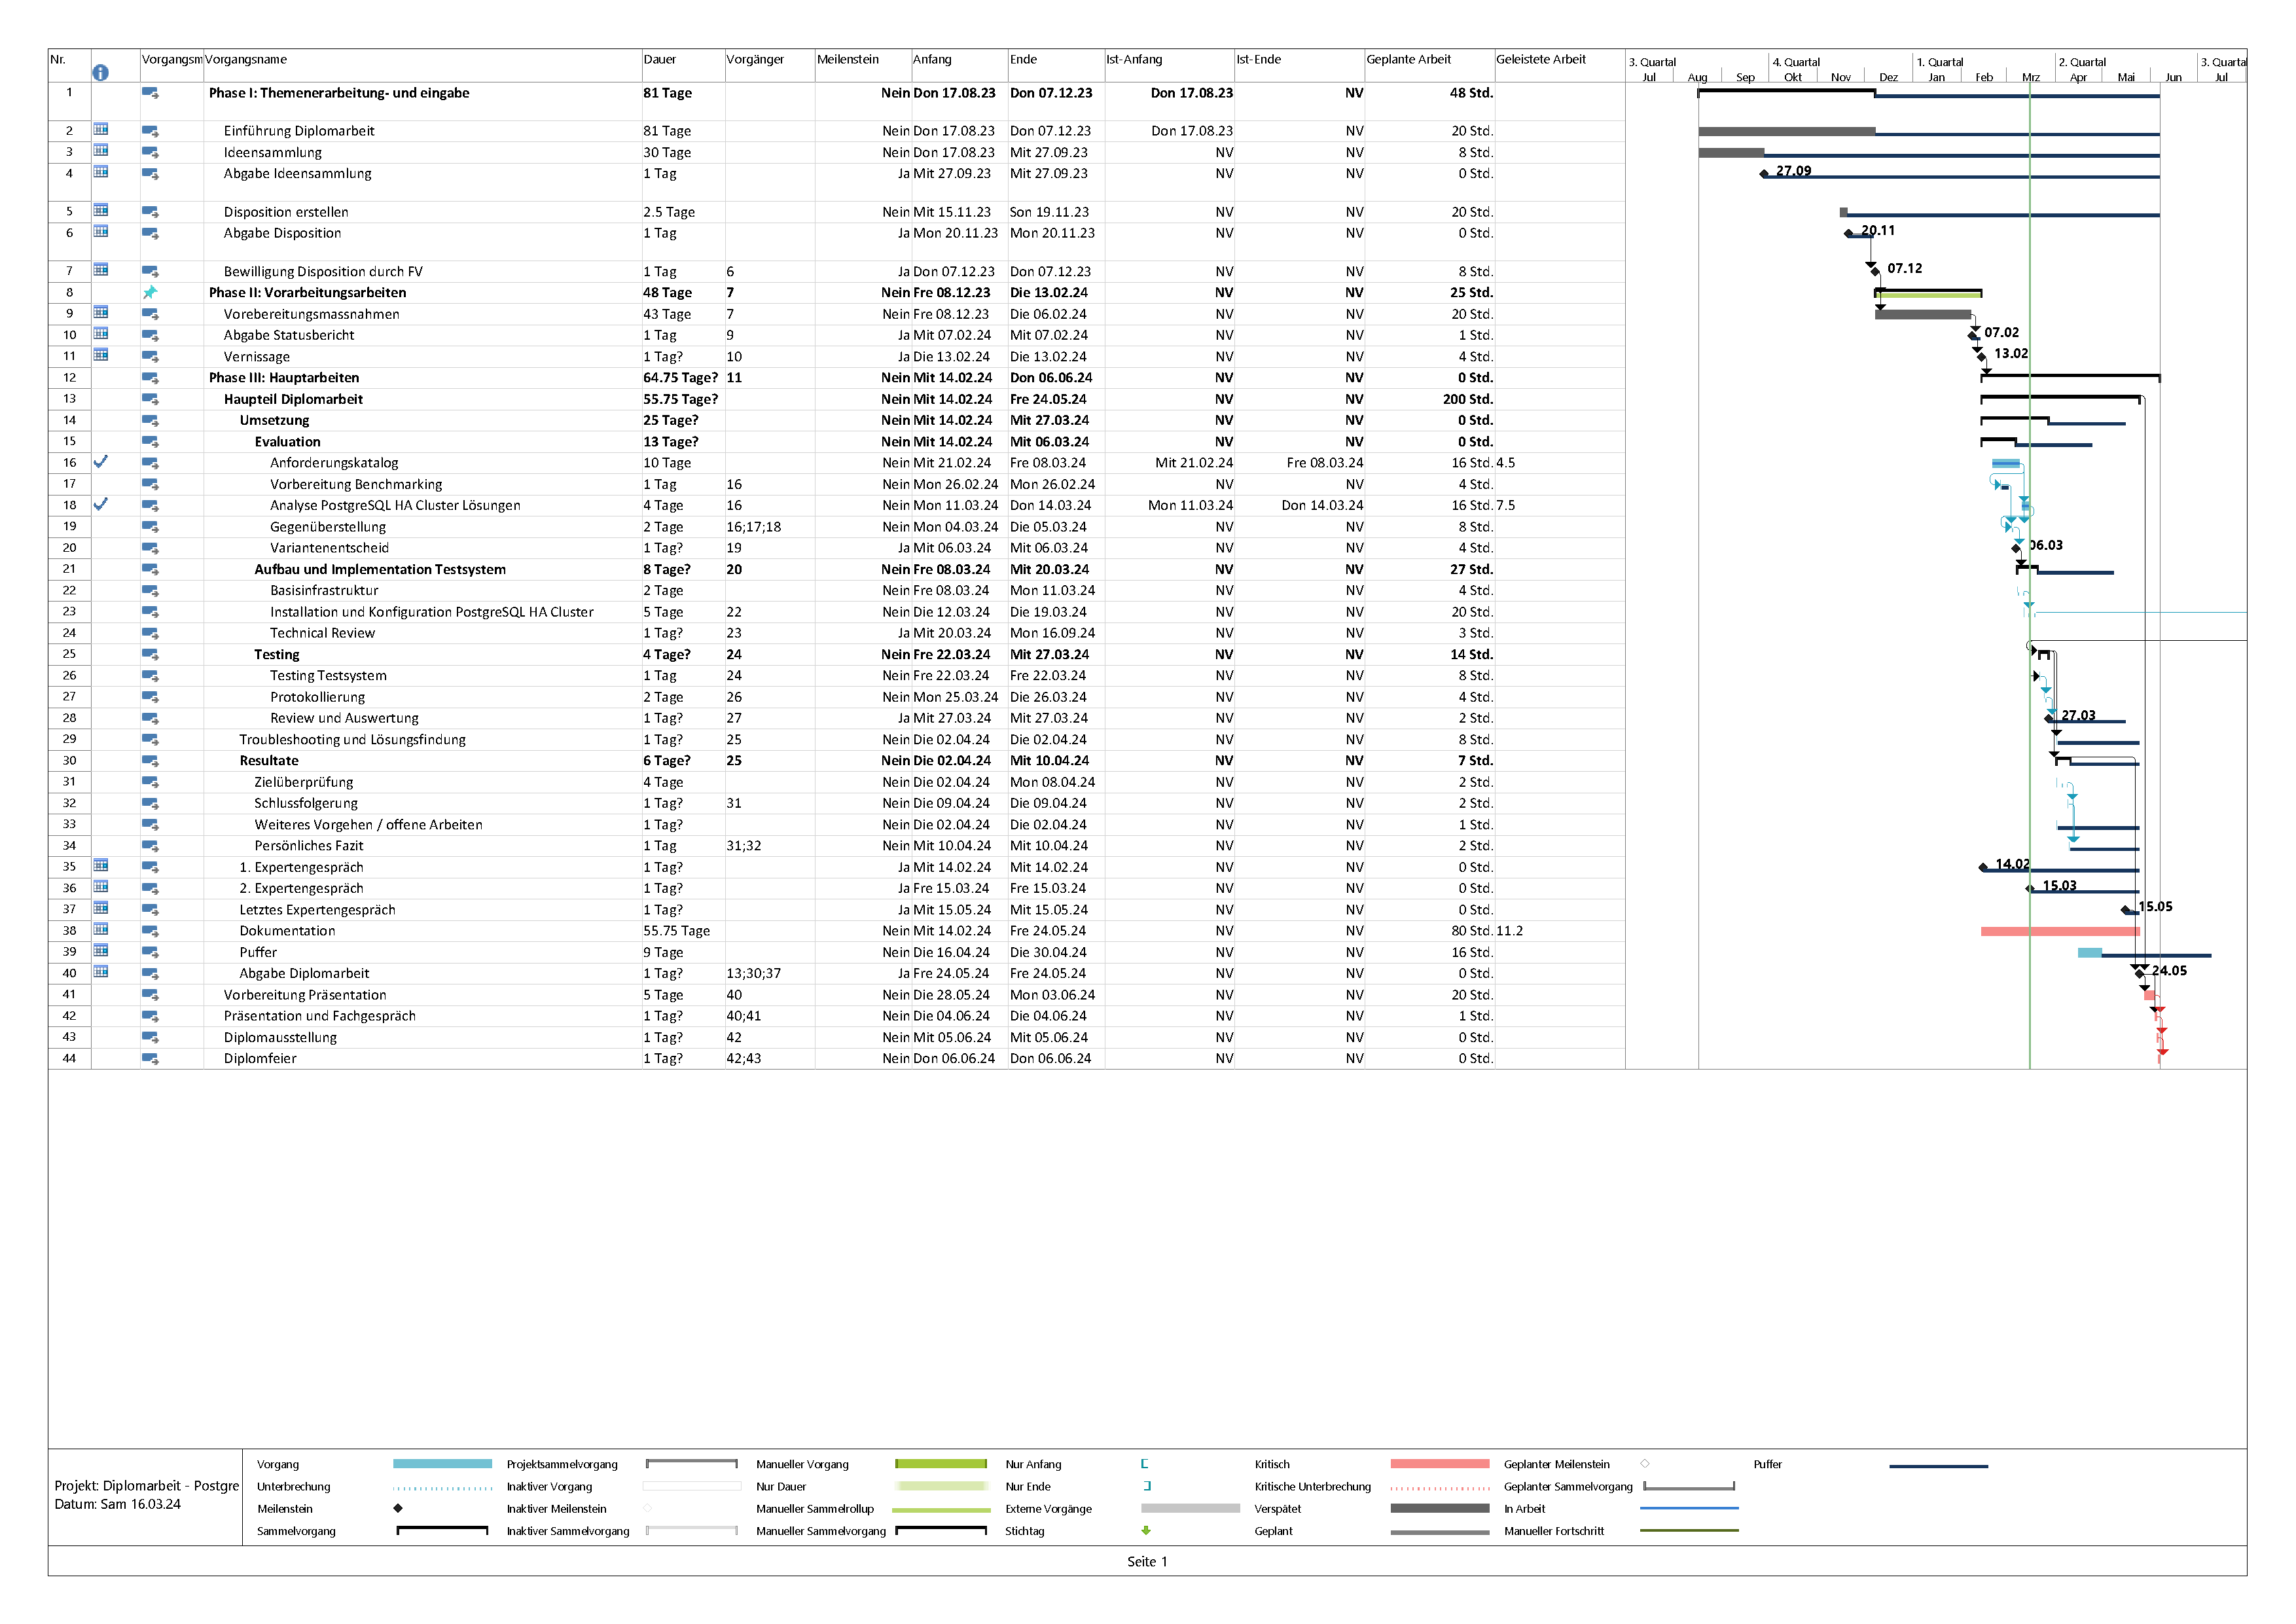
\includepdf[pages={1-},scale=1,landscape=true]{source/status_report/main/Diplomarbeit - PostgreSQL HA Cluster - Konzeption und Implementation - 2.pdf}
%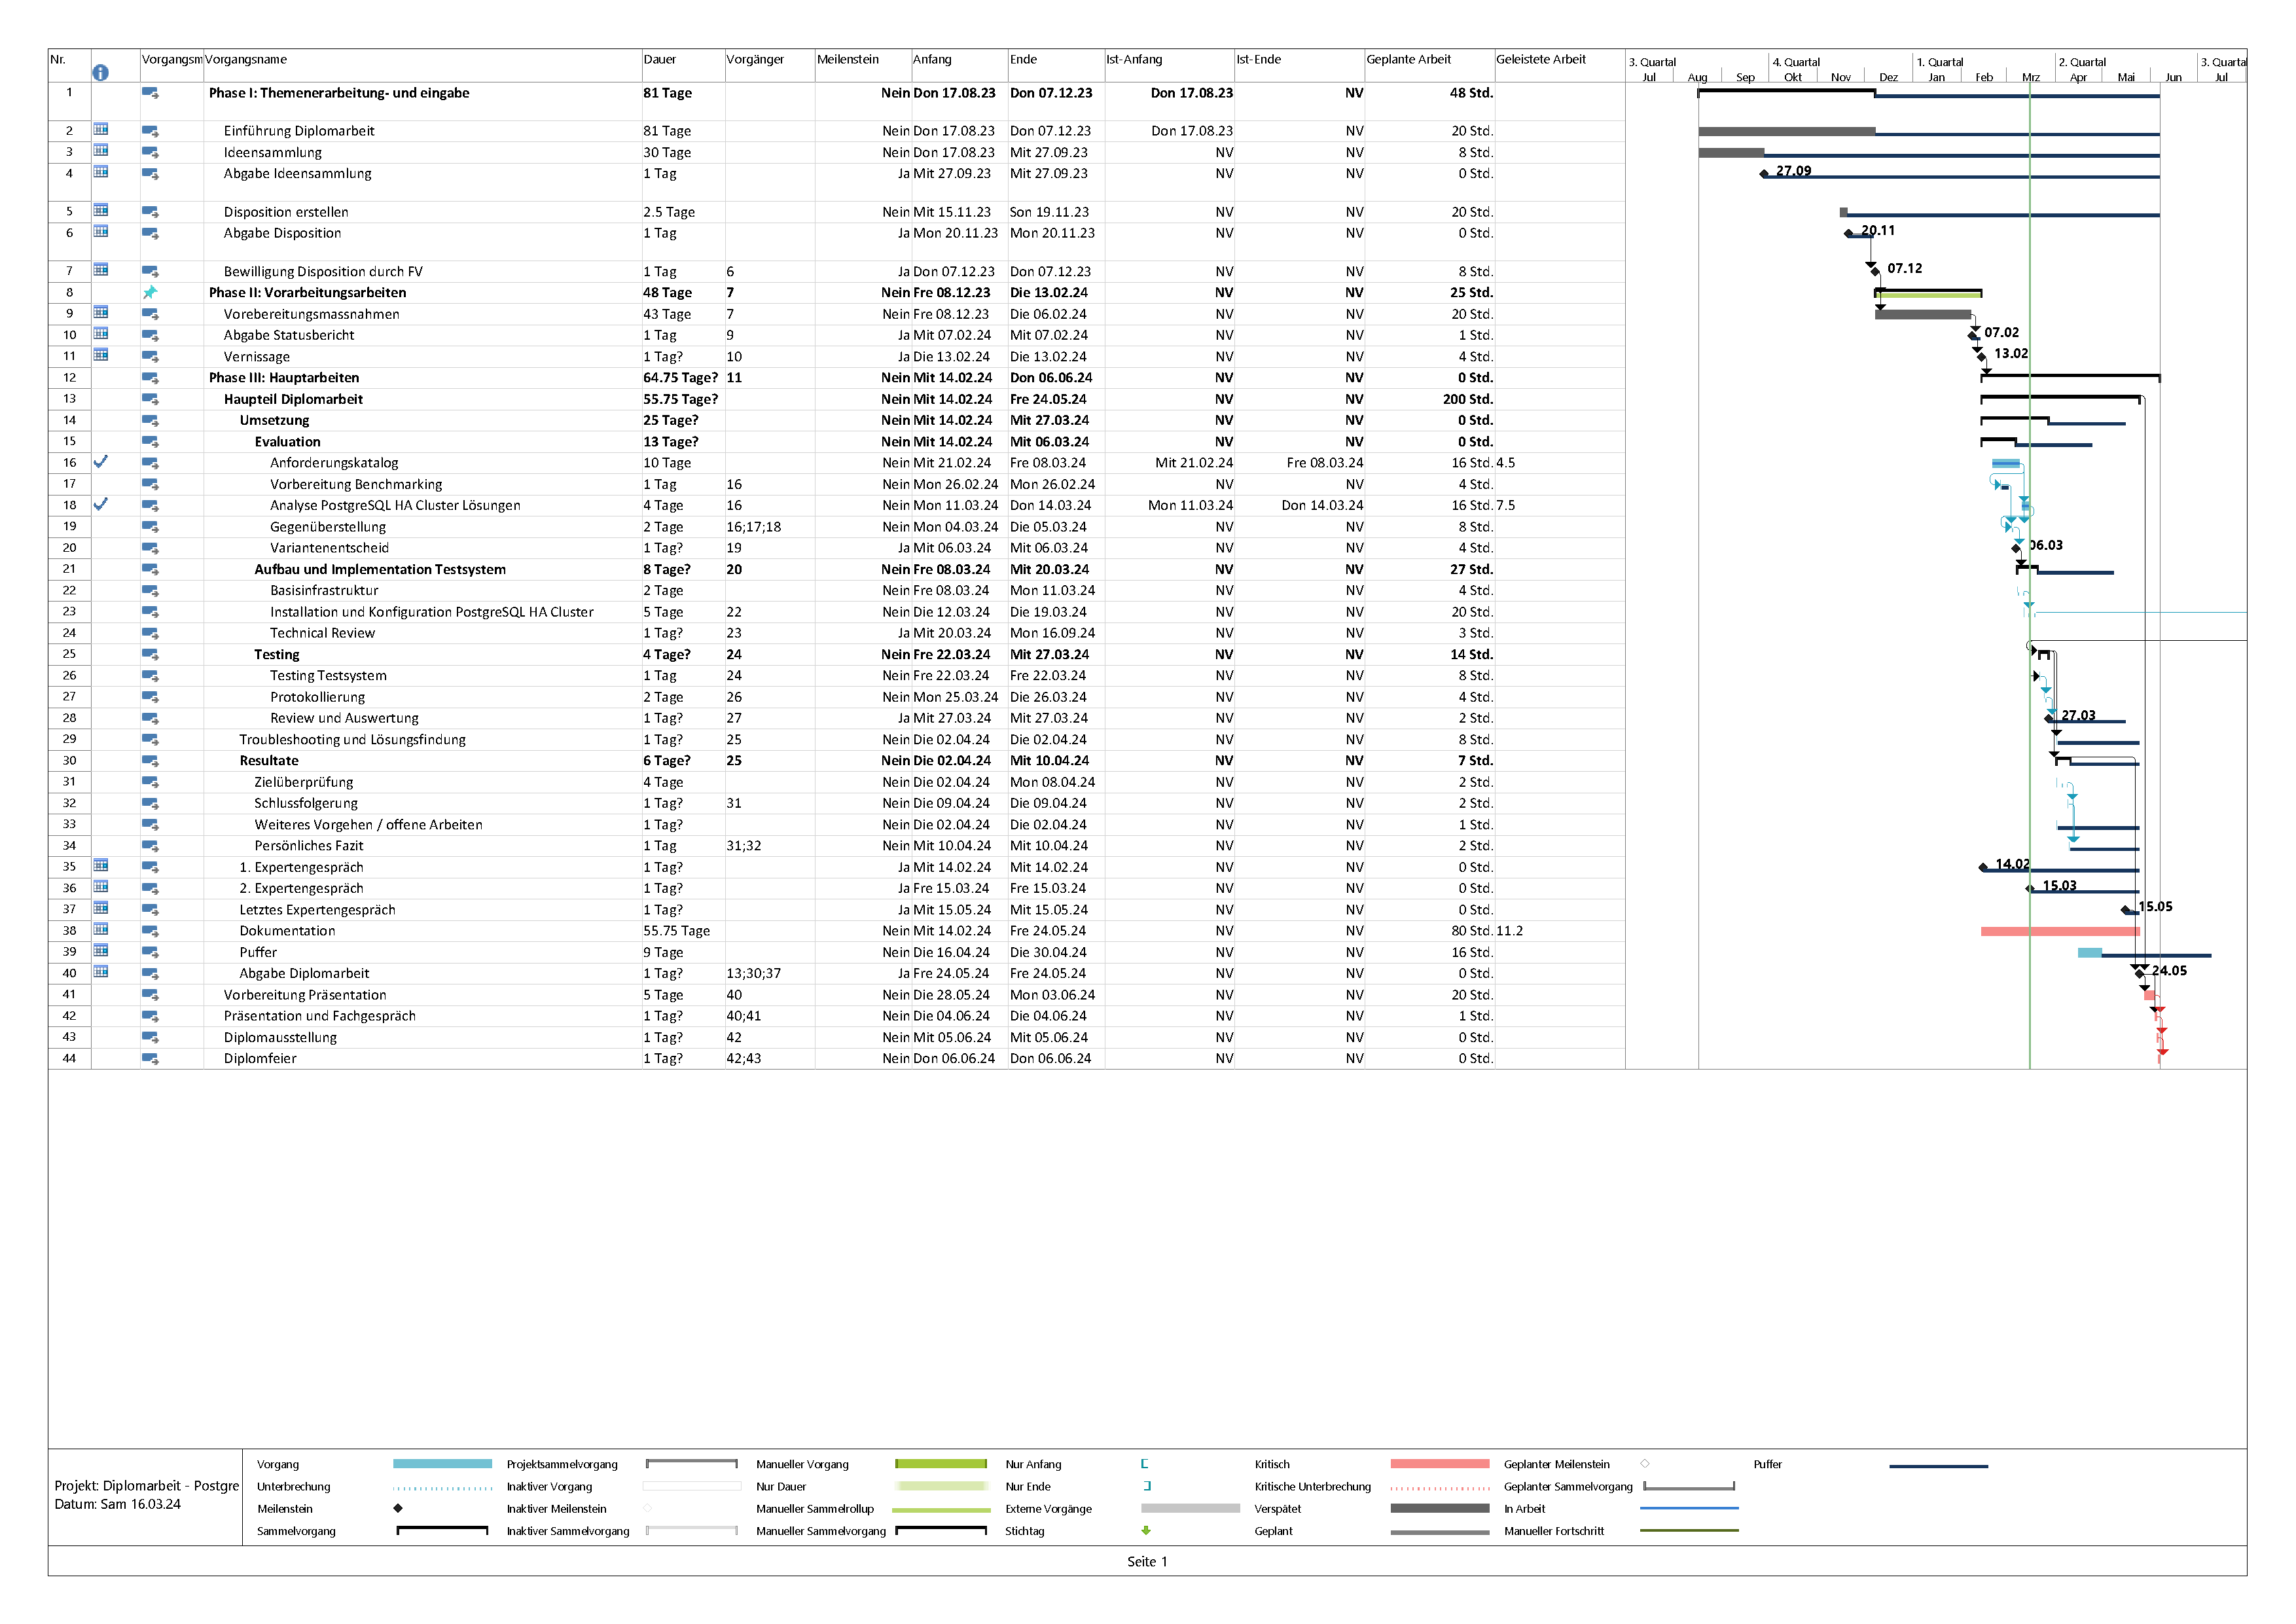
\includepdf[pages={1-,pagecommand={\subsection{GANTT-Diagramm}}, fitpaper=true,scale=0.8]{source/status_report/main/Diplomarbeit - PostgreSQL HA Cluster - Konzeption und Implementation - 2.pdf}


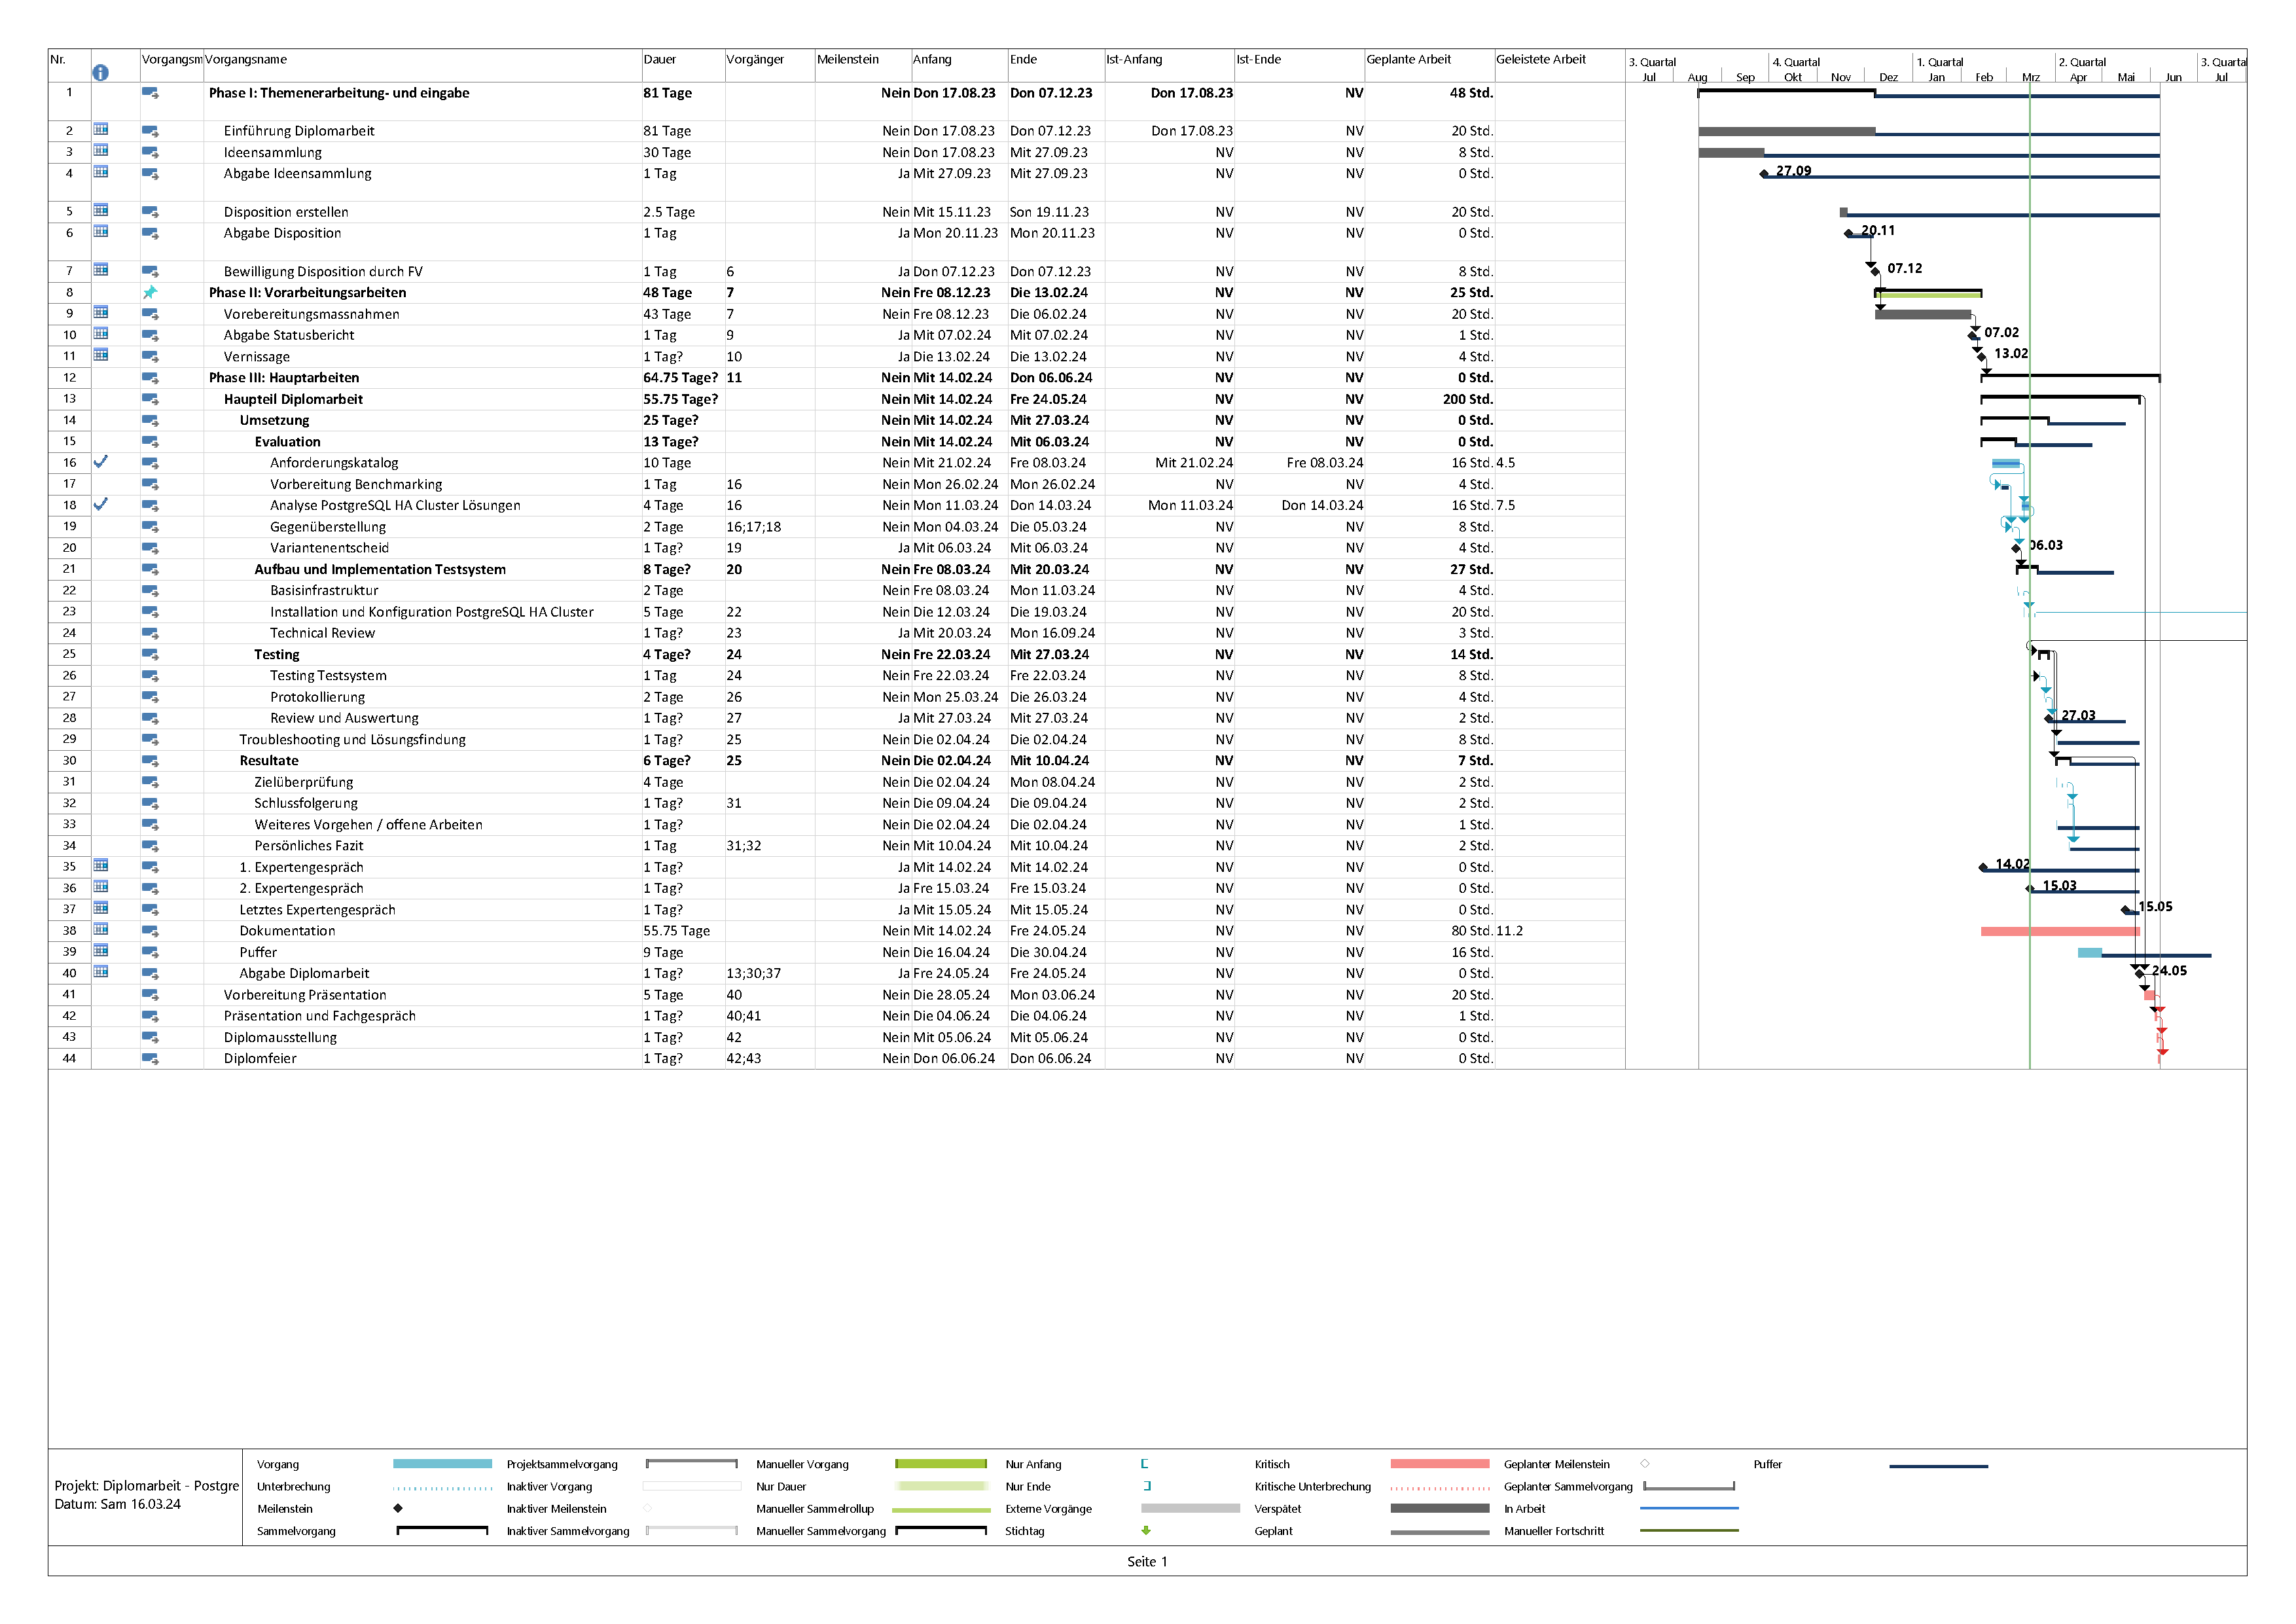
\includepdf[pages=1-,pagecommand={\subsection{GANTT-Diagramm}}, fitpaper=true,scale=0.9]{source/status_report/main/Diplomarbeit - PostgreSQL HA Cluster - Konzeption und Implementation - 2.pdf}
%\end{samepage}
%\KOMAoptions{paper=A3,paper=landscape,DIV=20}
%\setuppapersize[A4]
%\stoptext
%\KOMAoptions{paper=A4,paper=portrait,DIV=calc}
%\recalctypearea
%\end{landscape}

%\begin{landscape}
%\end{landscape}
%%! Author = itgramic
%! Date = 23.02.24

% Preamble
\begin{flushleft}
    \begin{landscape}
    \section{Status-Reports}
    %! Author = itgramic
%! Date = 22.01.24

% Preamble
\subsection{Initialer Statusbericht}
\begin{table}[H]
\centering
\resizebox{\textwidth}{!}{%
\begin{tabular}{lllllll}
\rowcolor[HTML]{C00000}
\multicolumn{5}{l}{\cellcolor[HTML]{C00000}{\color[HTML]{FFFFFF} \textbf{\begin{tabular}[c]{@{}l@{}}PostgreSQL HA Cluster - Konzeption und Implementation\end{tabular}}}}                                                                                                                                                                                                                                                                                                                                                                               & {\color[HTML]{FFFFFF} \textbf{ICT Projektstatusberich}}                                                                                                                    & {\color[HTML]{FFFFFF} \textbf{13.02.2024}}                                                                             \\
\cellcolor[HTML]{A6A6A6}{\color[HTML]{FFFFFF} \textbf{Projektbeschreibung}} & \multicolumn{4}{l}{Evaluation und Implementation PostgreSQL HA Cluster}                                                                                                                                                                                                                                                                                                                                                                                                     & \cellcolor[HTML]{A6A6A6}{\color[HTML]{FFFFFF} \textbf{Priorität}}                                                                                                          &                                                                                                                        \\ \hline
\cellcolor[HTML]{A6A6A6}{\color[HTML]{FFFFFF} \textbf{ICT veratw. Person}}  & \multicolumn{4}{l}{Michael Graber}                                                                                                                                                                                                                                                                                                                                                                                                                                          & \cellcolor[HTML]{A6A6A6}{\color[HTML]{FFFFFF} \textbf{PMA}}                                                                                                                & -                                                                                                                      \\ \hline
\multicolumn{7}{l}{}                                                                                                                                                                                                                                                                                                                                                                                                                                                                                                                                                                                                                                                                                                                                                                                                                                            \\
\multicolumn{7}{c}{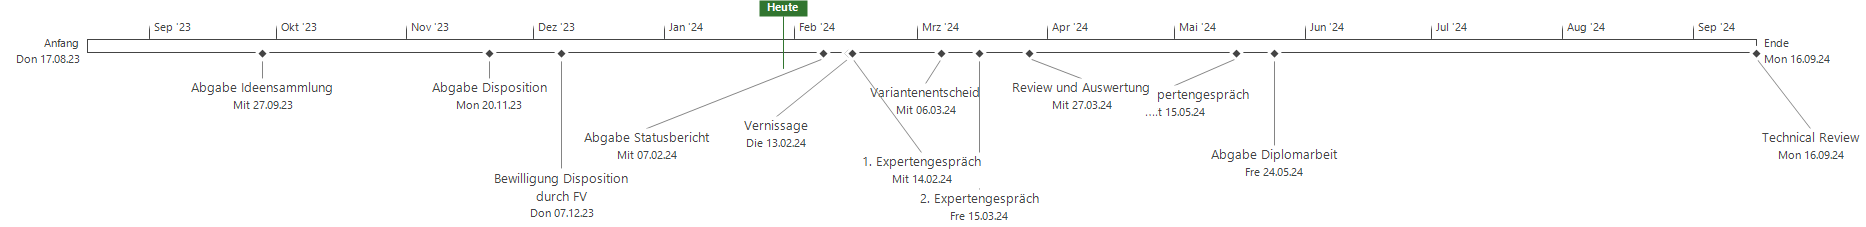
\includegraphics[width=2\linewidth]{source/status_report/main/init_timeline}}                                                                                                                                                                                                                                                                                                                                                                                                                                                                                                                                                                                                                                                                                                                                                                                                                                            \\
\multicolumn{7}{l}{}                                                                                                                                                                                                                                                                                                                                                                                                                                                                                                                                                                                                                                                                                                                                                                                                                                            \\
\rowcolor[HTML]{A6A6A6}
{\color[HTML]{FFFFFF} Status}                                               & {\color[HTML]{FFFFFF} Ampel}                                                                                                               & {\color[HTML]{FFFFFF} Tendenz}                                                                                                               & {\color[HTML]{FFFFFF} } & \multicolumn{3}{l}{\cellcolor[HTML]{A6A6A6}{\color[HTML]{FFFFFF} Begründung}}                                                                                                                                                                                                                                                                                                                                                                               \\
\textbf{Gesamtprojekt}                                                      & \multicolumn{1}{c}{}                                                                                                                       & \multicolumn{1}{c}{}                                                                                                                         &                         & \multicolumn{3}{l}{}                                                                                                                                                                                                                                                                                                                                                                                                                                        \\ \hline
Zeitplanung                                                                 & \multicolumn{1}{c}{{
\includegraphics[width=0.02\linewidth]{source/status_report/main/red}}}         & \multicolumn{1}{c}{{
\includegraphics[width=0.02\linewidth]{source/status_report/main/worse}}}         &                         & \multicolumn{3}{l}{Projekt ist Umfangreich und hat viele Teilaspekte, die es zu planen und berücksichtigen gilt}                                                                                                                                                                                                                                                                                                                                            \\ \hline
Ressourcen                                                                  & \multicolumn{1}{c}{{
\includegraphics[width=0.02\linewidth]{source/status_report/main/orange}}}      & \multicolumn{1}{c}{{
\includegraphics[width=0.02\linewidth]{source/status_report/main/worse}}}         &                         & \multicolumn{3}{l}{\begin{tabular}[c]{@{}l@{}}Parallel läuft das Grossprojket "Erneuerung HP UX Plattform", wo die bestehende HP-UX Plattform durch eine Oracle Exadata Cloud@Customer Plattform abgelöst wird.\\ Ab dem Zeitpunkt der Lieferung der Hardware werden die Oracle Datenbanken der Kernapplikation auf die neue Plattform migriert.\\ Dies über das gesamte Jahr und auch während der Diplomarbeit sehr viele Ressourcen binden.\end{tabular}} \\ \hline
Kosten                                                                      & \multicolumn{1}{c}{{
\includegraphics[width=0.02\linewidth]{source/status_report/main/green}}} & \multicolumn{1}{c}{{
\includegraphics[width=0.02\linewidth]{source/status_report/main/stagnation}}}    &                         & \multicolumn{3}{l}{Kosten sind noch im Soll-Bereich}                                                                                                                                                                                                                                                                                                                                                                                                        \\ \hline
\multicolumn{7}{l}{\textbf{}}                                                                                                                                                                                                                                                                                                                                                                                                                                                                                                                                                                                                                                                                                                                                                                                                                                   \\
\multicolumn{3}{l}{\cellcolor[HTML]{A6A6A6}{\color[HTML]{FFFFFF} \textbf{Tätigkeiten vergangene Berichtsperiode}}}                                                                                                                                                                                                                                                      &                         & \multicolumn{3}{l}{\cellcolor[HTML]{A6A6A6}{\color[HTML]{FFFFFF} Tätigkeiten nächste Berichtsperiode}}                                                                                                                                                                                                                                                                                                                                                      \\
\multicolumn{3}{l}{\begin{tabular}[c]{@{}l@{}}- Dokumentenstruktur erstellt\\ - Projektplanung erstellt\\ - Versnissage vorbereitet\\ - Statusbericht erstellt\end{tabular}}                                                                                                                                                                                            &                         & \multicolumn{3}{l}{\begin{tabular}[c]{@{}l@{}}- Anforderungskatalog erarbeiten\\ - Vorbereitung Benchmarking\end{tabular}}                                                                                                                                                                                                                                                                                                                                  \\ \cline{1-3} \cline{5-7}
\multicolumn{7}{l}{}                                                                                                                                                                                                                                                                                                                                                                                                                                                                                                                                                                                                                                                                                                                                                                                                                                            \\
\multicolumn{3}{l}{\cellcolor[HTML]{A6A6A6}{\color[HTML]{FFFFFF} \# nächste Lieferobjekte (inkl. allfällige Links)}}                                                                                                                                                                                                                                                    &                         & \cellcolor[HTML]{A6A6A6}{\color[HTML]{FFFFFF} Status}                                                                                                 & \cellcolor[HTML]{A6A6A6}{\color[HTML]{FFFFFF} Erledigungsgrad}                                                                                                             & \cellcolor[HTML]{A6A6A6}{\color[HTML]{FFFFFF} Soll Datum}                                                              \\
LO-001                                                                      & \multicolumn{2}{l}{Anforderungskatalog}                                                                                                                                                                                                                                                   &                         & in arbeit                                                                                                                                                 & \progressbar[heighta=10pt,width=3cm,ticksheight=0,linecolor=olive,tickscolor=black,emptycolor= white,filledcolor=olive]{0.6} \textbf{60\%}                                                      &         23.02.2024                                                                                                               \\
LO-002                                                                      & \multicolumn{2}{l}{Vorbereiten Benchmarking}                                                                                                                                                                                                                                              &                         & in arbeit                                                                                                                                                 & \progressbar[heighta=10pt,width=3cm,ticksheight=0,linecolor=olive,tickscolor=black,emptycolor= white,filledcolor=olive]{0} \textbf{0\%}                                                              &    26.02.2024                                                                                                                    \\
LO-003                                                                      & \multicolumn{2}{l}{}                                                                                                                                                                                                                                                                      &                         &                                                                                                                                                       &                                                                                                                                                                            &                                                                                                                        \\
LO-004                                                                      & \multicolumn{2}{l}{}                                                                                                                                                                                                                                                                      &                         &                                                                                                                                                       &                                                                                                                                                                            &                                                                                                                        \\
LO-005                                                                      & \multicolumn{2}{l}{}                                                                                                                                                                                                                                                                      &                         &                                                                                                                                                       &                                                                                                                                                                            &                                                                                                                        \\ \cline{1-3} \cline{5-7}
\multicolumn{7}{l}{}                                                                                                                                                                                                                                                                                                                                                                                                                                                                                                                                                                                                                                                                                                                                                                                                                                            \\
\rowcolor[HTML]{A6A6A6}
\multicolumn{2}{l}{\cellcolor[HTML]{A6A6A6}{\color[HTML]{FFFFFF} \# Risiken}}                                                                                                                                            & {\color[HTML]{FFFFFF} Auswirkungsgrad}                                                                                                       &                         & {\color[HTML]{FFFFFF} Massnahmen}                                                                                                                     & {\color[HTML]{FFFFFF} }                                                                                                                                                    & {\color[HTML]{FFFFFF} Verantw.}                                                                                        \\
R-001                                                                       & Fehlende Ressourcen                                                                                                                        & \multicolumn{1}{c}{{
\includegraphics[width=0.02\linewidth]{source/status_report/main/risk_warning}}} &                         & Organisation und Selbstmanagement                                                                                                                     &                                                                                                                                                                            &                                                                                                                        \\ \hline
R-002                                                                       & HP-UX Ablöseprojekt                                                                                                                        & \multicolumn{1}{c}{{
\includegraphics[width=0.02\linewidth]{source/status_report/main/risk_alert}}}                       &                         & Ressourcen reservieren                                                                                                                                &                                                                                                                                                                            &                                                                                                                        \\ \hline
R-003                                                                       & Alte Infrastruktur kann ungeplant sämtliche Ressourcen binden                                                                              & \multicolumn{1}{c}{{
\includegraphics[width=0.02\linewidth]{source/status_report/main/risk_alert}}}                       &                         & Monitoring vorgängig ausbauen und Massnahmen definieren                                                                                               &                                                                                                                                                                            &                                                                                                                        \\ \hline
R-004                                                                       & Schwächen beim Selbstmanagement und in der Selbstorganisation                                                                              & \multicolumn{1}{c}{{
\includegraphics[width=0.02\linewidth]{source/status_report/main/risk_warning}}}                     &                         & Werkzeuge im Vorfeld definieren und bereitstellen                                                                                                     &                                                                                                                                                                            &                                                                                                                        \\ \hline
                                                                            &                                                                                                                                            &                                                                                                                                              &                         &                                                                                                                                                       &                                                                                                                                                                            &                                                                                                                        \\
\multicolumn{3}{l}{\cellcolor[HTML]{A6A6A6}{\color[HTML]{FFFFFF} Kostenübersicht}}                                                                                                                                                                                                                                                                                      &                         & \cellcolor[HTML]{A6A6A6}{\color[HTML]{FFFFFF} Abhängigkeiten zu anderen Projekten}                                                                    & \multicolumn{2}{l}{\cellcolor[HTML]{A6A6A6}{\color[HTML]{FFFFFF} Massnahmen}}                                                                                                                                                                                                                       \\
\multicolumn{3}{l}{}                                                                                                                                                                                                                                                                                                                                                    &                         & Erneuerung HP UX Plattform 60002201                                                                                                                   & \multicolumn{2}{l}{Ressourcen reservieren}                                                                                                                                                                                                                                                          \\
\multicolumn{3}{l}{\multirow{-2}{*}{\begin{tabular}[c]{@{}l@{}}Verfügbare Finanzen bis Ende Projekt:\\ \(\frac{\SI{100}{\CHF}}{h} * 200h = \SI{24000}{\CHF}\)\end{tabular}}}                                                                                                                                                                                              &                         & KSGR Provisioning System (KPS) =\textgreater Foreman Umgebung                                                                                         & \multicolumn{2}{l}{Massnahmen ergreifen um die manuelle Installation so effizient wie möglich zu gestalten}                                                                                                                                                                                         \\ \cline{1-3} \cline{5-7}
                                                                            &                                                                                                                                            &                                                                                                                                              &                         &                                                                                                                                                       &                                                                                                                                                                            &                                                                                                                        \\
\multicolumn{3}{l}{\cellcolor[HTML]{A6A6A6}{\color[HTML]{FFFFFF} Bemerkungen / Informationen}}                                                                                                                                                                                                                                                                          &                         & \multicolumn{3}{l}{\cellcolor[HTML]{A6A6A6}{\color[HTML]{FFFFFF} Anträge}}                                                                                                                                                                                                                                                                                                                                                                                  \\
\multicolumn{3}{l}{}                                                                                                                                                                                                                                                                                                                                                    &                         & \multicolumn{3}{l}{}                                                                                                                                                                                                                                                                                                                                                                                                                                        \\ \cline{1-3} \cline{5-7}
\multicolumn{7}{l}{}                                                                                                                                                                                                                                                                                                                                                                                                                                                                                                                                                                                                                                                                                                                                                                                                                                            \\
\cellcolor[HTML]{A6A6A6}{\color[HTML]{FFFFFF} Eingereicht}                  & \cellcolor[HTML]{A6A6A6}{\color[HTML]{FFFFFF} }                                                                                            & \cellcolor[HTML]{A6A6A6}{\color[HTML]{FFFFFF} Geprüft}                                                                                       &                         & \multicolumn{3}{l}{\cellcolor[HTML]{A6A6A6}{\color[HTML]{FFFFFF} Bemerkungen/Auftrag PMO}}                                                                                                                                                                                                                                                                                                                                                                  \\
\multicolumn{2}{l}{PL:}                                                                                                                                                                                                  & PMO:                                                                                                                                         &                         & \multicolumn{3}{l}{}                                                                                                                                                                                                                                                                                                                                                                                                                                        \\
\multicolumn{2}{l}{Datum:}                                                                                                                                                                                               & Datum:                                                                                                                                       &                         & \multicolumn{3}{l}{}                                                                                                                                                                                                                                                                                                                                                                                                                                        \\ \cline{1-3} \cline{5-7}
\multicolumn{7}{l}{}                                                                                                                                                                                                                                                                                                                                                                                                                                                                                                                                                                                                                                                                                                                                                                                                                                            \\
\multicolumn{7}{l}{\multirow{-2}{*}{}}                                                                                                                                                                                                                                                                                                                                                                                                                                                                                                                                                                                                                                                                                                                                                                                                                          \\
\rowcolor[HTML]{A6A6A6}
\multicolumn{7}{l}{\cellcolor[HTML]{A6A6A6}{\color[HTML]{FFFFFF} \# erledigte Lieferobjekte (inkl. allfällige Links)}}                                                                                                                                                                                                                                                                                                                                                                                                                                                                                                                                                                                                                                                                                                                                          \\
\multicolumn{7}{l}{}
\end{tabular}%
}
\caption{Initialer Statusbericht}
\label{tab:init_status_report}
\end{table}
%\end{landscape}
    %! Author = gramic
%! Date = 16.03.24

% Preamble
\subsection{Zweiter Statusbericht}
\begin{table}[H]
\centering
\resizebox{\textwidth}{!}{%
\begin{tabular}{lllllll}
\rowcolor[HTML]{C00000}
\multicolumn{5}{l}{\cellcolor[HTML]{C00000}{\color[HTML]{FFFFFF} \textbf{PostgreSQL HA Cluster - Konzeption und Implementation}}}                                                                                                                                                                                                                                                                                                                                                  & {\color[HTML]{FFFFFF} \textbf{ICT Projektstatusberich}}                                                                                                         & {\color[HTML]{FFFFFF} \textbf{18.03.2024}}                                                                                      \\
\cellcolor[HTML]{A6A6A6}{\color[HTML]{FFFFFF} \textbf{Projektbeschreibung}} & \multicolumn{4}{l}{Evaluation und Implementation PostgreSQL HA Cluster}                                                                                                                                                                                                                                                                                                                              & \cellcolor[HTML]{A6A6A6}{\color[HTML]{FFFFFF} \textbf{Priorität}}                                                                                               &                                                                                                                                 \\ \hline
\cellcolor[HTML]{A6A6A6}{\color[HTML]{FFFFFF} \textbf{ICT veratw. Person}}  & \multicolumn{4}{l}{Michael Graber}                                                                                                                                                                                                                                                                                                                                                                   & \cellcolor[HTML]{A6A6A6}{\color[HTML]{FFFFFF} \textbf{PMA}}                                                                                                     & -                                                                                                                               \\ \hline
\multicolumn{7}{l}{}                                                                                                                                                                                                                                                                                                                                                                                                                                                                                                                                                                                                                                                                                                                                                                   \\
\multicolumn{7}{l}{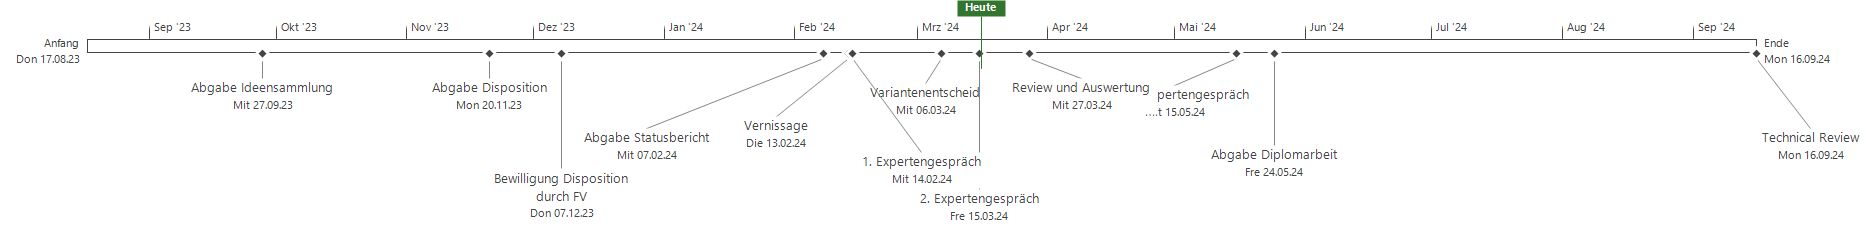
\includegraphics[width=2\linewidth]{source/status_report/main/second_report_timeline}}                                                                                                                                                                                                                                                                                                                                                                                                                                                                                                                                                                                                                                                                           \\
\multicolumn{7}{l}{}                                                                                                                                                                                                                                                                                                                                                                                                                                                                                                                                                                                                                                                                                                                                                                   \\
\rowcolor[HTML]{A6A6A6}
{\color[HTML]{FFFFFF} Status}                                               & {\color[HTML]{FFFFFF} Ampel}                                                                       & {\color[HTML]{FFFFFF} Tendenz}                                                                       & {\color[HTML]{FFFFFF} } & \multicolumn{3}{l}{\cellcolor[HTML]{A6A6A6}{\color[HTML]{FFFFFF} Begründung}}                                                                                                                                                                                                                                                                                                                                                                                      \\
\textbf{Gesamtprojekt}                                                      & \multicolumn{1}{c}{}                                                                               & \multicolumn{1}{c}{}                                                                                 &                         & \multicolumn{3}{l}{}                                                                                                                                                                                                                                                                                                                                                                                                                                               \\ \hline
Zeitplanung                                                                 & \multicolumn{1}{c}{{
\includegraphics[width=0.05\linewidth]{source/status_report/main/red}}}        & \multicolumn{1}{c}{{
\includegraphics[width=0.05\linewidth]{source/status_report/main/worse}}}        &                         & \multicolumn{3}{l}{\begin{tabular}[c]{@{}l@{}}In verzug.\\ Grossprojket \texttt{Erneuerung HP UX Plattform} nimmt viel Zeit in Anschlag.\\ Hinzu kommt, das die analyse gängiger PostgreSQL HA Lösungen ebenfalls viel Zeit kostet.\\ Dokumentionsaufwand unterschätzt.\end{tabular}}                                                                                                                                                                              \\ \hline
Ressourcen                                                                  & \multicolumn{1}{c}{{
\includegraphics[width=0.05\linewidth]{source/status_report/main/orange}}}     & \multicolumn{1}{c}{{
\includegraphics[width=0.05\linewidth]{source/status_report/main/worse}}}        &                         & \multicolumn{3}{l}{\begin{tabular}[c]{@{}l@{}}Parallel läuft das Grossprojket \texttt{Erneuerung HP UX Plattform}, wo die bestehende HP-UX Plattform durch eine Oracle Exadata Cloud@Customer Plattform abgelöst wird.\\ Ab dem Zeitpunkt der Lieferung der Hardware werden die Oracle Datenbanken der Kernapplikation auf die neue Plattform migriert.\\ Dies über das gesamte Jahr und auch während der Diplomarbeit sehr viele Ressourcen binden.\end{tabular}} \\ \hline
Kosten                                                                      & \multicolumn{1}{c}{{
\includegraphics[width=0.05\linewidth]{source/status_report/main/risk_alert}}} & \multicolumn{1}{c}{{
\includegraphics[width=0.05\linewidth]{source/status_report/main/stagnation}}}   &                         & \multicolumn{3}{l}{Kosten sind noch im Soll-Bereich}                                                                                                                                                                                                                                                                                                                                                                                                               \\ \hline
\multicolumn{7}{l}{\textbf{}}                                                                                                                                                                                                                                                                                                                                                                                                                                                                                                                                                                                                                                                                                                                                                          \\
\multicolumn{3}{l}{\cellcolor[HTML]{A6A6A6}{\color[HTML]{FFFFFF} \textbf{Tätigkeiten vergangene Berichtsperiode}}}                                                                                                                                                                      &                         & \multicolumn{3}{l}{\cellcolor[HTML]{A6A6A6}{\color[HTML]{FFFFFF} Tätigkeiten nächste Berichtsperiode}}                                                                                                                                                                                                                                                                                                                                                             \\
\multicolumn{3}{l}{\begin{tabular}[c]{@{}l@{}}- Anforderungskatalog erstellt\\ - Parallel dokumentiert\end{tabular}}                                                                                                                                                                    &                         & \multicolumn{3}{l}{\begin{tabular}[c]{@{}l@{}}- Analyse der PostgreSQL HA Clusterlösungen abgeschlossen\\ - Benchmarking abgeschlossen \\ - Variantenentscheid getroffen\\ - Basissystem für Testsystem aufgebaut\end{tabular}}                                                                                                                                                                                                                                    \\ \cline{1-3} \cline{5-7}
\multicolumn{7}{l}{}                                                                                                                                                                                                                                                                                                                                                                                                                                                                                                                                                                                                                                                                                                                                                                   \\
\multicolumn{3}{l}{\cellcolor[HTML]{A6A6A6}{\color[HTML]{FFFFFF} \# nächste Lieferobjekte (inkl. allfällige Links)}}                                                                                                                                                                     &                         & \cellcolor[HTML]{A6A6A6}{\color[HTML]{FFFFFF} Status}                                                                                                          & \cellcolor[HTML]{A6A6A6}{\color[HTML]{FFFFFF} Erledigungsgrad}                                                                                                  & \cellcolor[HTML]{A6A6A6}{\color[HTML]{FFFFFF} Soll Datum}                                                                       \\
LO-002                                                                      & \multicolumn{2}{l}{Vorbereiten Benchmarking}                                                                                                                                                              &                         & offen                                                                                                                                                          & \progressbar[linecolor=blue,tickscolor=orange,emptycolor= white,filledcolor=green]{0}                                                                           &                                                                                                                                 \\
LO-003                                                                      & \multicolumn{2}{l}{Analyse PostgreSQL HA Cluster Lösungen}                                                                                                                                                &                         & in Arbeit                                                                                                                                                      & \progressbar[linecolor=blue,tickscolor=orange,emptycolor= white,filledcolor=orange]{0.4}                                                                        &                                                                                                                                 \\
LO-004                                                                      & \multicolumn{2}{l}{Gegenüberstellung}                                                                                                                                                                     &                         & offen                                                                                                                                                          & \progressbar[linecolor=blue,tickscolor=orange,emptycolor= white,filledcolor=green]{0}                                                                           &                                                                                                                                 \\
LO-005                                                                      & \multicolumn{2}{l}{Variantenentscheid}                                                                                                                                                                    &                         & offen                                                                                                                                                          & \progressbar[linecolor=blue,tickscolor=orange,emptycolor= white,filledcolor=green]{0}                                                                           &                                                                                                                                 \\
LO-006                                                                      & \multicolumn{2}{l}{Aufbau Basisinfrakstruktur Testsystem}                                                                                                                                                 &                         & offen                                                                                                                                                          & \progressbar[linecolor=blue,tickscolor=orange,emptycolor= white,filledcolor=green]{0}                                                                           &                                                                                                                                 \\ \cline{1-3} \cline{5-7}
\multicolumn{7}{l}{}                                                                                                                                                                                                                                                                                                                                                                                                                                                                                                                                                                                                                                                                                                                                                                   \\
\rowcolor[HTML]{A6A6A6}
\multicolumn{2}{l}{\cellcolor[HTML]{A6A6A6}{\color[HTML]{FFFFFF} \# Risiken}}                                                                                                     & {\color[HTML]{FFFFFF} Auswirkungsgrad}                                                               &                         & {\color[HTML]{FFFFFF} Massnahmen}                                                                                                                              & {\color[HTML]{FFFFFF} }                                                                                                                                         & {\color[HTML]{FFFFFF} Verantw.}                                                                                                 \\
R-001                                                                       & Fehlende Ressourcen                                                                                & \multicolumn{1}{c}{{
\includegraphics[width=0.05\linewidth]{source/status_report/main/risk_warning}}} &                         & Organisation und Selbstmanagement                                                                                                                              &                                                                                                                                                                 &                                                                                                                                 \\ \hline
R-002                                                                       & HP-UX Ablöseprojekt                                                                                & {
\includegraphics[width=0.05\linewidth]{source/status_report/main/risk_alert}}                       &                         & Ressourcen reservieren                                                                                                                                         &                                                                                                                                                                 &                                                                                                                                 \\ \hline
R-003                                                                       & Alte Infrastruktur kann ungeplant sämtliche Ressourcen binden                                      & {
\includegraphics[width=0.05\linewidth]{source/status_report/main/risk_alert}}                       &                         & Monitoring vorgängig ausbauen und Massnahmen definieren                                                                                                        &                                                                                                                                                                 &                                                                                                                                 \\ \hline
R-004                                                                       & Schwächen beim Selbstmanagement und in der Selbstorganisation                                      & {
\includegraphics[width=0.05\linewidth]{source/status_report/main/risk_warning}}                     &                         & Werkzeuge im Vorfeld definieren und bereitstellen                                                                                                              &                                                                                                                                                                 &                                                                                                                                 \\ \hline
R-005                                                                       & Scope verlust während des Projekts                                                                 & {
\includegraphics[width=0.05\linewidth]{source/status_report/main/risk_warning}}                     &                         & Ziele klar definieren                                                                                                                                          &                                                                                                                                                                 &                                                                                                                                 \\ \hline
R-006                                                                       & Scope Creep                                                                                        & {
\includegraphics[width=0.05\linewidth]{source/status_report/main/risk_warning}}                     &                         & Ziele SMART definieren                                                                                                                                         &                                                                                                                                                                 &                                                                                                                                 \\ \hline
R-007                                                                       & SIEM / Log Plattform nicht betriebsbereit                                                          & {
\includegraphics[width=0.05\linewidth]{source/status_report/main/risk_warning}}                     &                         &                                                                                                                                                                &                                                                                                                                                                 &                                                                                                                                 \\ \hline
R-008                                                                       & Foreman nicht betriebsbereit                                                                       & {
\includegraphics[width=0.05\linewidth]{source/status_report/main/risk_warning}}                     &                         & Massnahmen ergreifen um die manuelle Installation so effizient wie möglich zu gestalten                                                                        &                                                                                                                                                                 &                                                                                                                                 \\ \hline
                                                                            &                                                                                                    &                                                                                                      &                         &                                                                                                                                                                &                                                                                                                                                                 &                                                                                                                                 \\
\multicolumn{3}{l}{\cellcolor[HTML]{A6A6A6}{\color[HTML]{FFFFFF} Kostenübersicht}}                                                                                                                                                                                                      &                         & \cellcolor[HTML]{A6A6A6}{\color[HTML]{FFFFFF} Abhängigkeiten zu anderen Projekten}                                                                             & \multicolumn{2}{l}{\cellcolor[HTML]{A6A6A6}{\color[HTML]{FFFFFF} Massnahmen}}                                                                                                                                                                                                                     \\
\multicolumn{3}{l}{}                                                                                                                                                                                                                                                                    &                         & Erneuerung HP UX Plattform 60002201                                                                                                                            & \multicolumn{2}{l}{Ressourcen reservieren}                                                                                                                                                                                                                                                        \\
\multicolumn{3}{l}{\multirow{-2}{*}{\begin{tabular}[c]{@{}l@{}}Verfügbare Finanzen bis Ende Projekt:\\ \(\SI{100}{\CHF\per\hour} * 200 = \SI{24000}{\CHF}\)\end{tabular}}}                                                                                                              &                         & KSGR Provisioning System (KPS) => Foreman Umgebung                                                                                                             & \multicolumn{2}{l}{Massnahmen ergreifen um die manuelle Installation so effizient wie möglich zu gestalten}                                                                                                                                                                                       \\ \cline{1-3} \cline{5-7}
                                                                            &                                                                                                    &                                                                                                      &                         &                                                                                                                                                                &                                                                                                                                                                 &                                                                                                                                 \\
\multicolumn{3}{l}{\cellcolor[HTML]{A6A6A6}{\color[HTML]{FFFFFF} Bemerkungen / Informationen}}                                                                                                                                                                                          &                         & \multicolumn{3}{l}{\cellcolor[HTML]{A6A6A6}{\color[HTML]{FFFFFF} Anträge}}                                                                                                                                                                                                                                                                                                                                                                                         \\
\multicolumn{3}{l}{}                                                                                                                                                                                                                                                                    &                         & \multicolumn{3}{l}{}                                                                                                                                                                                                                                                                                                                                                                                                                                               \\ \cline{1-3} \cline{5-7}
\multicolumn{7}{l}{}                                                                                                                                                                                                                                                                                                                                                                                                                                                                                                                                                                                                                                                                                                                                                                   \\
\cellcolor[HTML]{A6A6A6}{\color[HTML]{FFFFFF} Eingereicht}                  & \cellcolor[HTML]{A6A6A6}{\color[HTML]{FFFFFF} }                                                    & \cellcolor[HTML]{A6A6A6}{\color[HTML]{FFFFFF} Geprüft}                                               &                         & \multicolumn{3}{l}{\cellcolor[HTML]{A6A6A6}{\color[HTML]{FFFFFF} Bemerkungen/Auftrag PMO}}                                                                                                                                                                                                                                                                                                                                                                         \\
\multicolumn{2}{l}{PL:}                                                                                                                                                          & PMO:                                                                                                 &                         & \multicolumn{3}{l}{}                                                                                                                                                                                                                                                                                                                                                                                                                                               \\
\multicolumn{2}{l}{Datum:}                                                                                                                                                       & Datum:                                                                                               &                         & \multicolumn{3}{l}{}                                                                                                                                                                                                                                                                                                                                                                                                                                               \\ \cline{1-3} \cline{5-7}
\multicolumn{7}{l}{}                                                                                                                                                                                                                                                                                                                                                                                                                                                                                                                                                                                                                                                                                                                                                                   \\
\multicolumn{7}{l}{\multirow{-2}{*}{}}                                                                                                                                                                                                                                                                                                                                                                                                                                                                                                                                                                                                                                                                                                                                                 \\
\rowcolor[HTML]{A6A6A6}
\multicolumn{7}{l}{\cellcolor[HTML]{A6A6A6}{\color[HTML]{FFFFFF} \# erledigte Lieferobjekte (inkl. allfällige Links)}}                                                                                                                                                                                                                                                                                                                                                                                                                                                                                                                                                                                                                                                                  \\
LO-001                                                                      & \multicolumn{2}{l}{Anforderungskatalog}                                                                                                                                                                   &                         & \multicolumn{3}{l}{}                                                                                                                                                                                                                                                                                                                                                                                                                                               \\ \cline{1-3} \cline{5-7}
\end{tabular}%
}
\caption{Zweiter Statusbericht}
\label{tab:second_status_report}
\end{table}
    \end{landscape}
\end{flushleft}

%\end{landscape}
%\noraml